\section{Earthquake Forecast Performance Measurements}
\label{sec:perf-main}



\subsection{Runtime}

\label{sec:perf-runtime}

implemented a GPU monitoring tool that has some features others did not have 
events
timer start, stop, status
with statements
summary table
info about cpus
various formats: table, json, csv


Timer revealed issue with one of the systems
\begin{verbatim}
StopWatch.event(“event-name”)

StopWatch.start(“name”)
StopWatch.stop(“name”)
StopWatch.status(“name”)

with StopWatchBlock(“name”)
      run_long_calculation()

@benchmark
	def f(...):
# decorator for function creates automatically start stop for that
# function, sums up all times for that function in run

StopWatch.benchmark() 
# prints the result in table, cvs and other formats (if needed)
\end{verbatim}

\subsection{Perfomance projection}



\begin{figure}[htb]
    \centering
    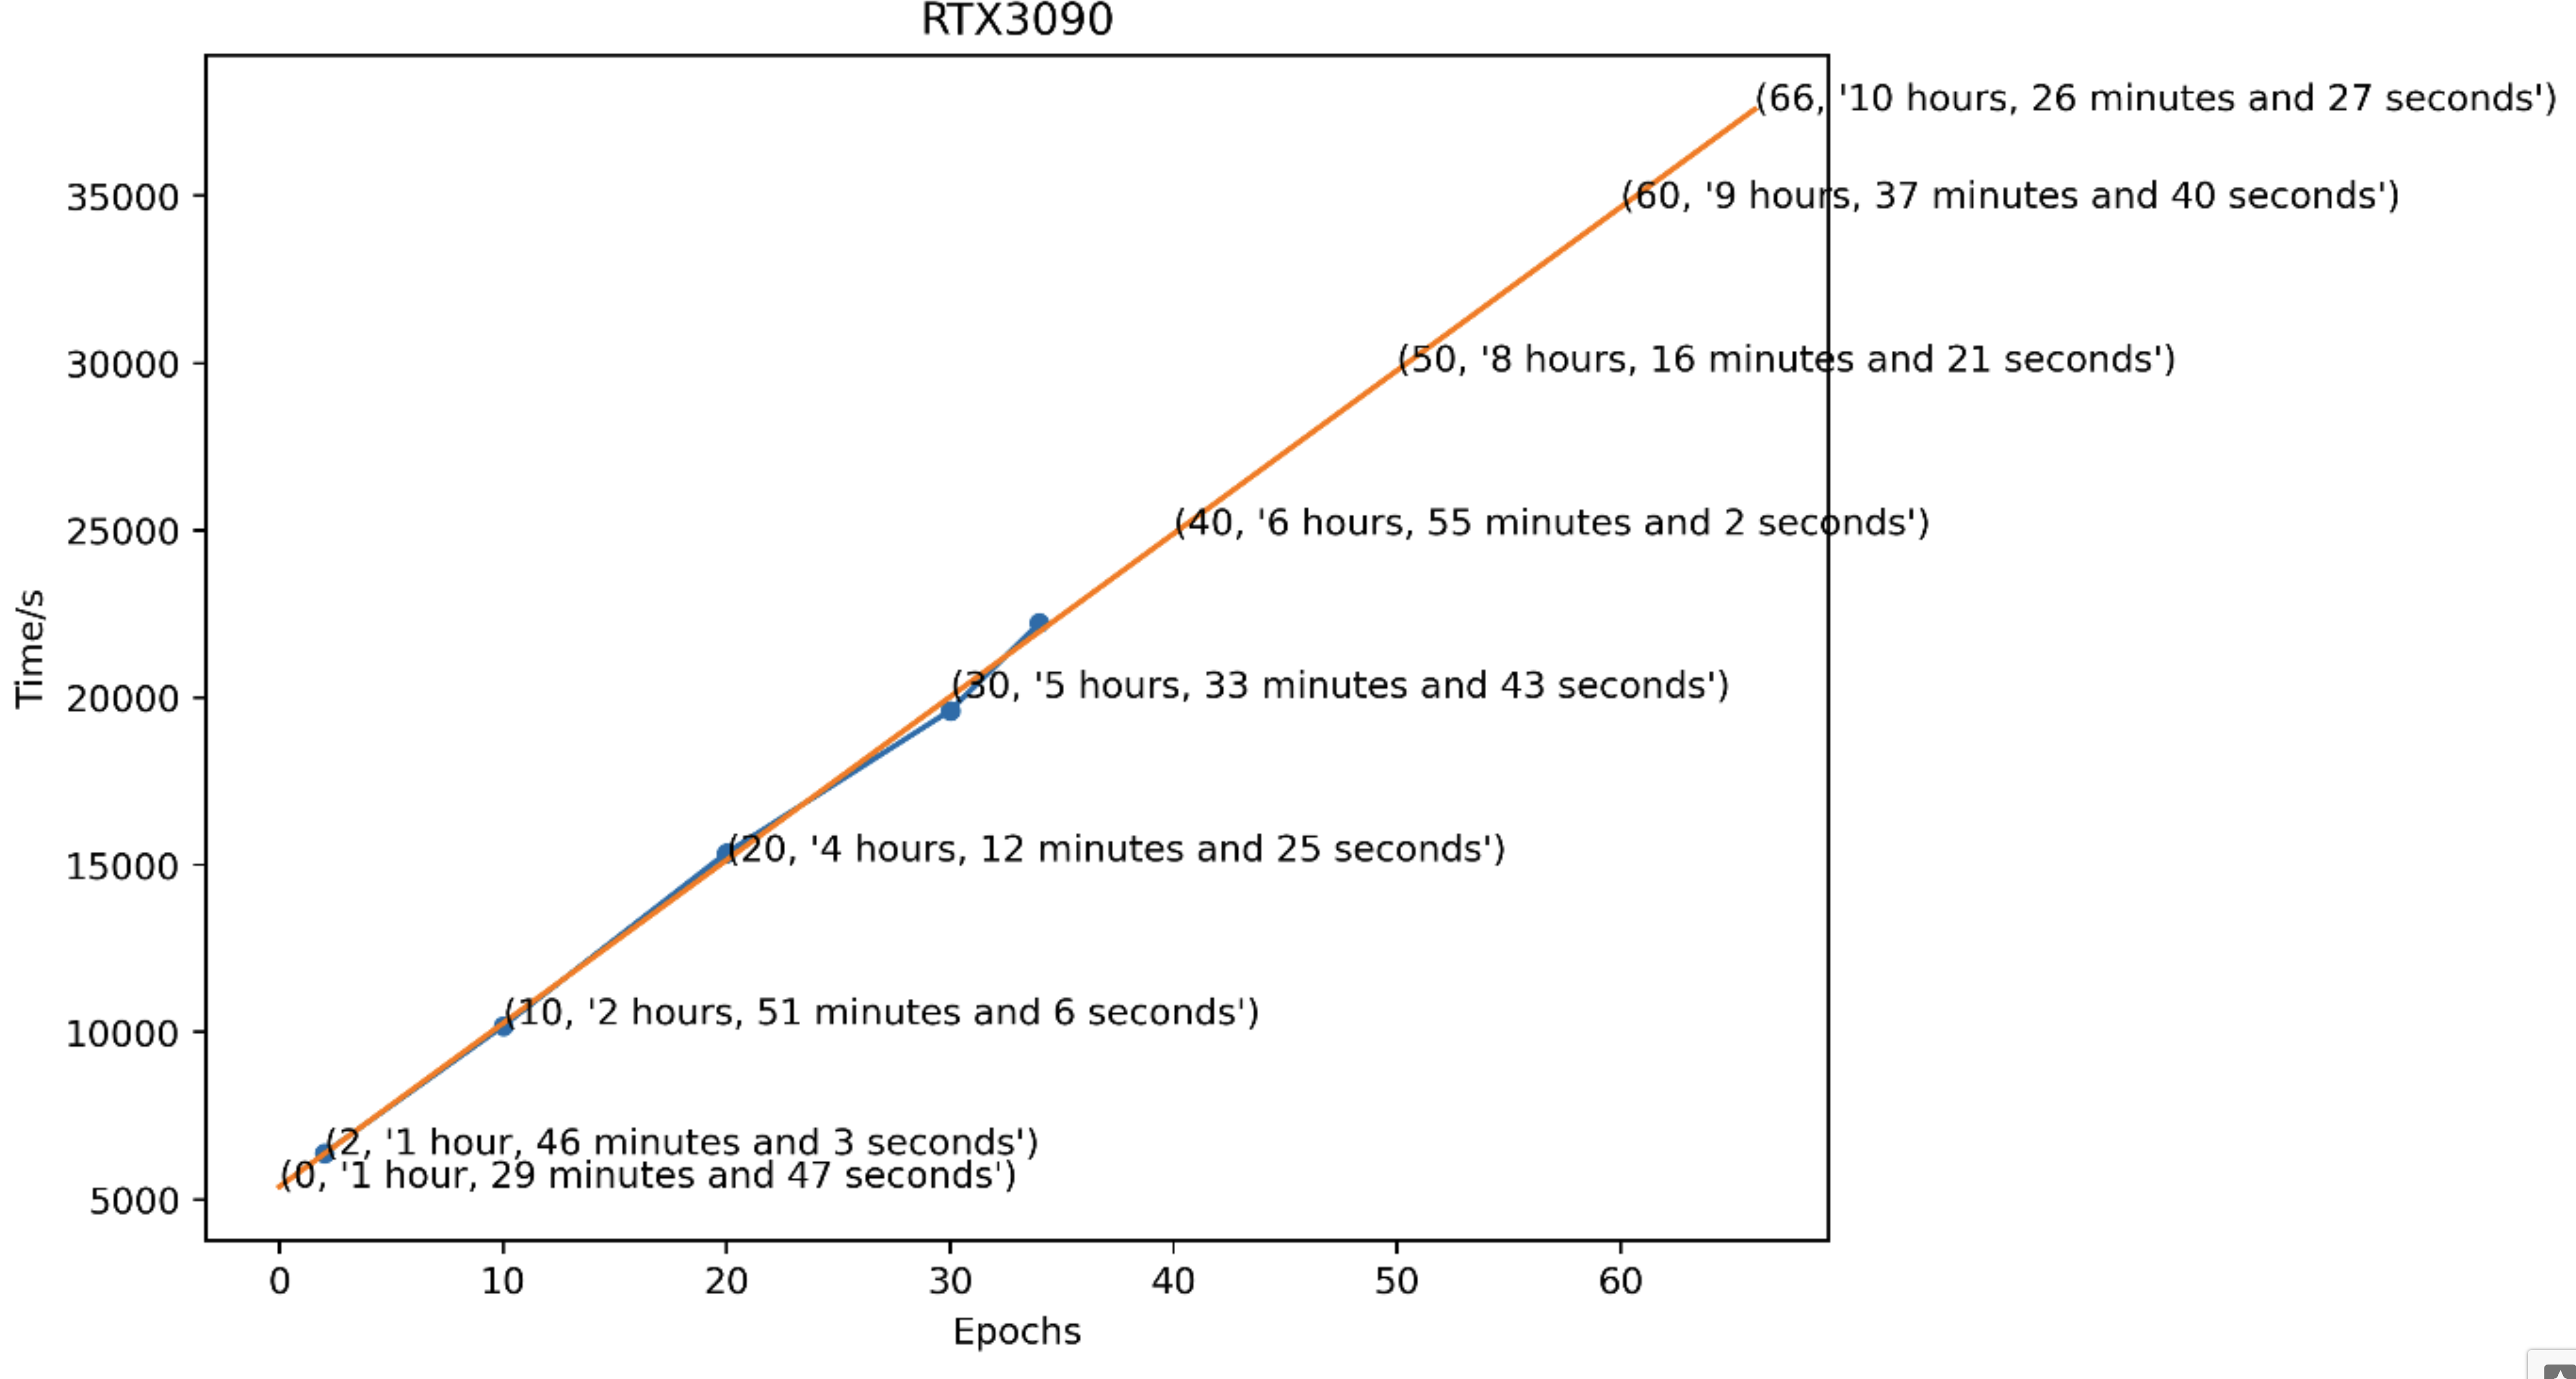
\includegraphics[width=0.70\columnwidth]{images/performance-projection.png}
    \caption{Performance projection. }
    \label{fig:performance-projection}
\end{figure}


\begin{figure}[htb]
    \centering
    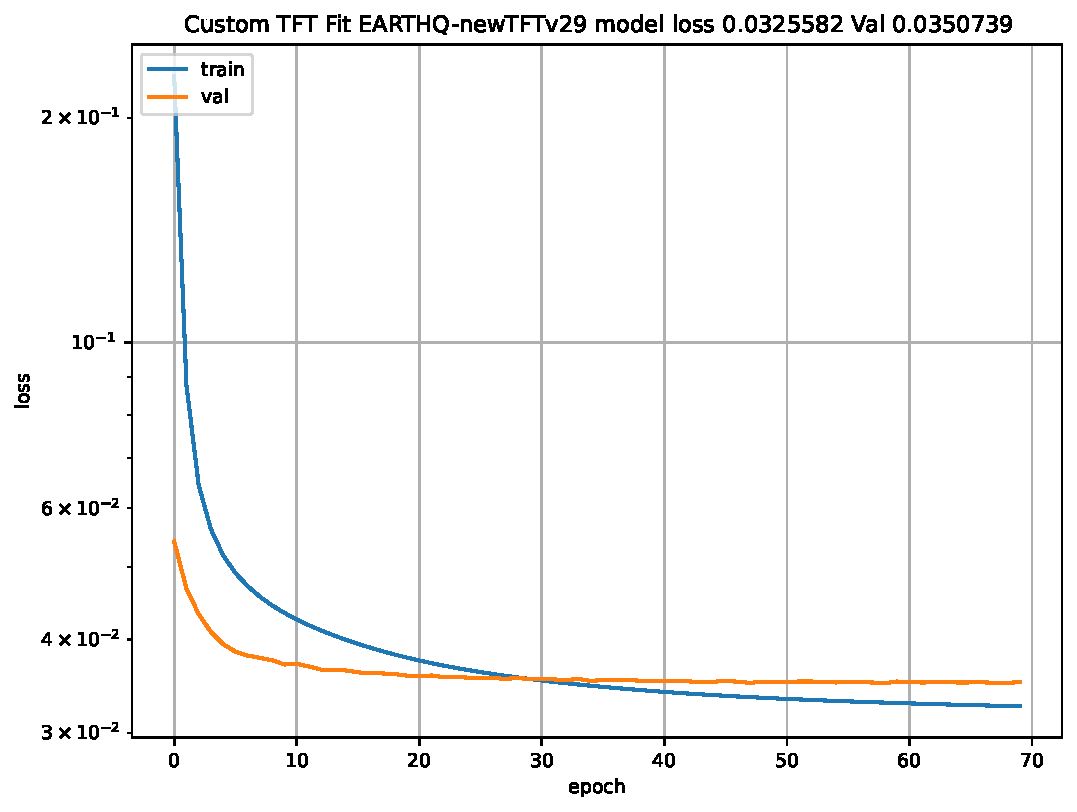
\includegraphics[width=0.70\columnwidth]{images/loss.png}
    \caption{Loss}
    \label{fig:loss}
  \end{figure}


  \begin{table}[htb]
    \caption{Runtime of the 2 epoch case in seconds}
    \LABEL{tab:2-epoch-case}
    {\footnotesize              
      \begin{center}
        \begin{table}[]
          \begin{tabular}{lrrrrr}
            Timer             & RTX3090 & RTX3080 & A100    & V100    & K80     \\
            \hline
            Machine           & Desktop & Laptop  & Rivanna & Rivanna & Rivanna \\
            Total             & 6589.4  & 8348.5  & 17574.8 & 20295.0 & 28343.3 \\
            Sampling location &  457.9  &  532.5  &  1227.0 &  1546.4 &  1779.6 \\
            Init              &    0.8  &    3.6  &    8.1  &     5.6 &     5.3 \\
            Train             & 1103.2  & 2068.9  &  1373.0 &  1671.4 &  6967.3 \\
            Bestfit           & 4420.3  & 4997.1  & 13022.1 & 14795.1 & 17037.6 \\
            \hline
          \end{tabular}
        \end{table}
        \end{center} 
    }
\end{table}

code management is important, github is essential
Need to have better sbatch to make code management easier
cluster design is important and access to local storage on nodes is important
shared file systems are less effective 
Predicting behavior of code is great with our timer library as it allows us to estimate runtines and report results in easy fashion. Helps debugging.
Need to look into the implementation of bestfit 
Need to look into memory dependency of epochs
Should we stop at 34 epochs or run 66?

\TODO{add k80 elsewher}

\begin{verbatim}
Cloudmesh Data Submodule - https://github.com/cloudmesh/cloudmesh-data
Cloudmesh GPU Submodule - https://github.com/cloudmesh/cloudmesh-gpu
Cloudmesh sbatch Submodule - https://github.com/cloudmesh/cloudmesh-sbatch 

\end{verbatim}


\subsection{Accuracy}

\label{sec:perf-accuracy}

%%% max 15 figures abd table, subfig is one figure

%%%  NB logo1.eps is required in the path in order to correctly compile front page header %%%



\begin{figure}[htb]

  \begin{center}

     \begin{minipage}[b]{0.45\textwidth}
       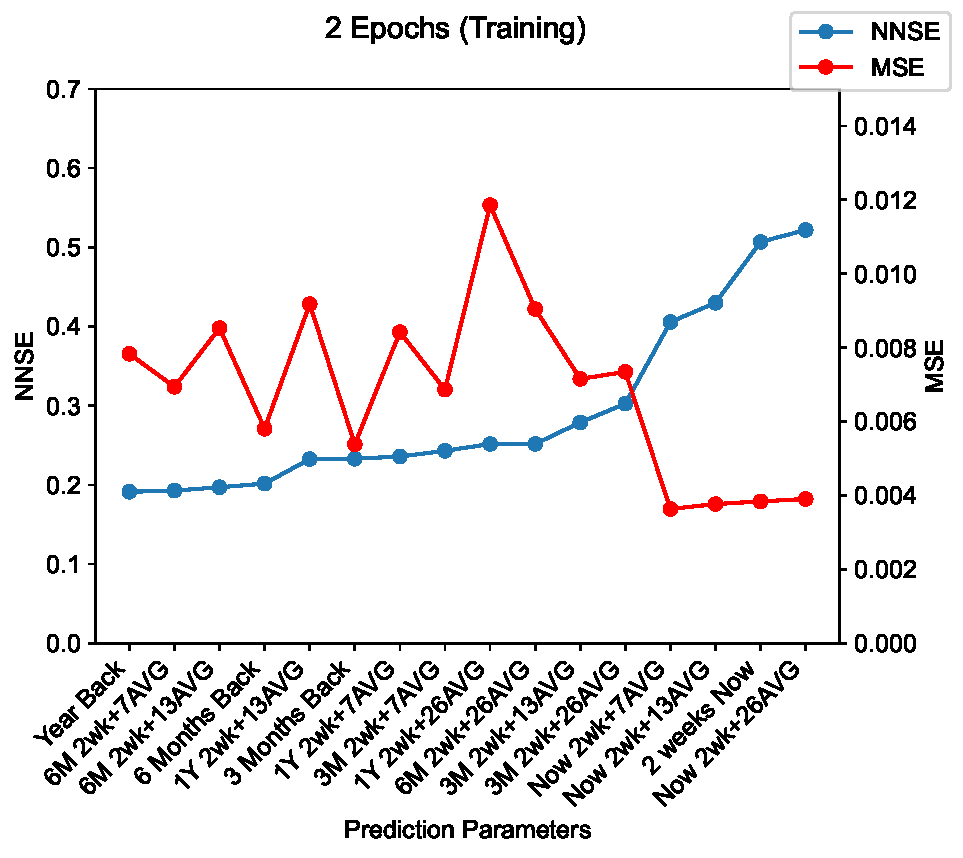
\includegraphics[width=1.0\linewidth]{images/2_training-MSE-and-NNSE.pdf}
        {\bf (A)} MSE and NNSE - 2 epochs training.
    \end{minipage}
     \ \
     \begin{minipage}[b]{0.45\textwidth}
        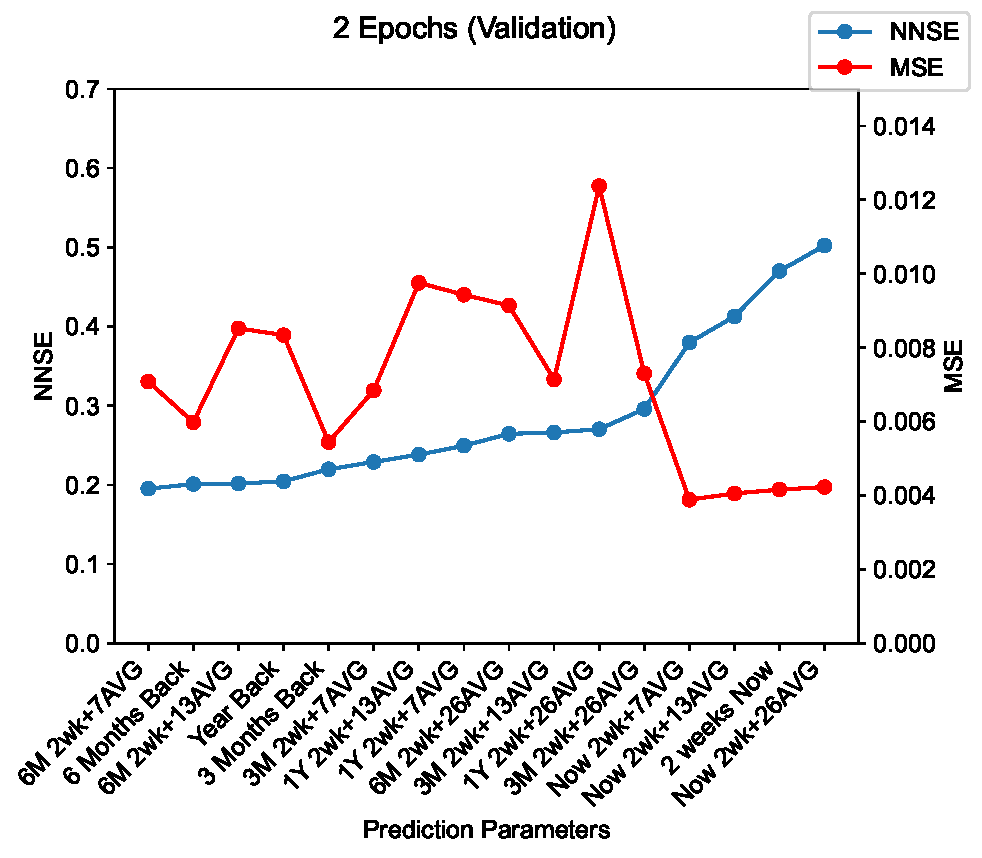
\includegraphics[width=1.0\linewidth]{images/2_validation-MSE-and-NNSE.pdf}
        {\bf (B)}  MSE and NNSE - 2 epochs validation.
     \end{minipage}

     \begin{minipage}[b]{0.45\textwidth}
        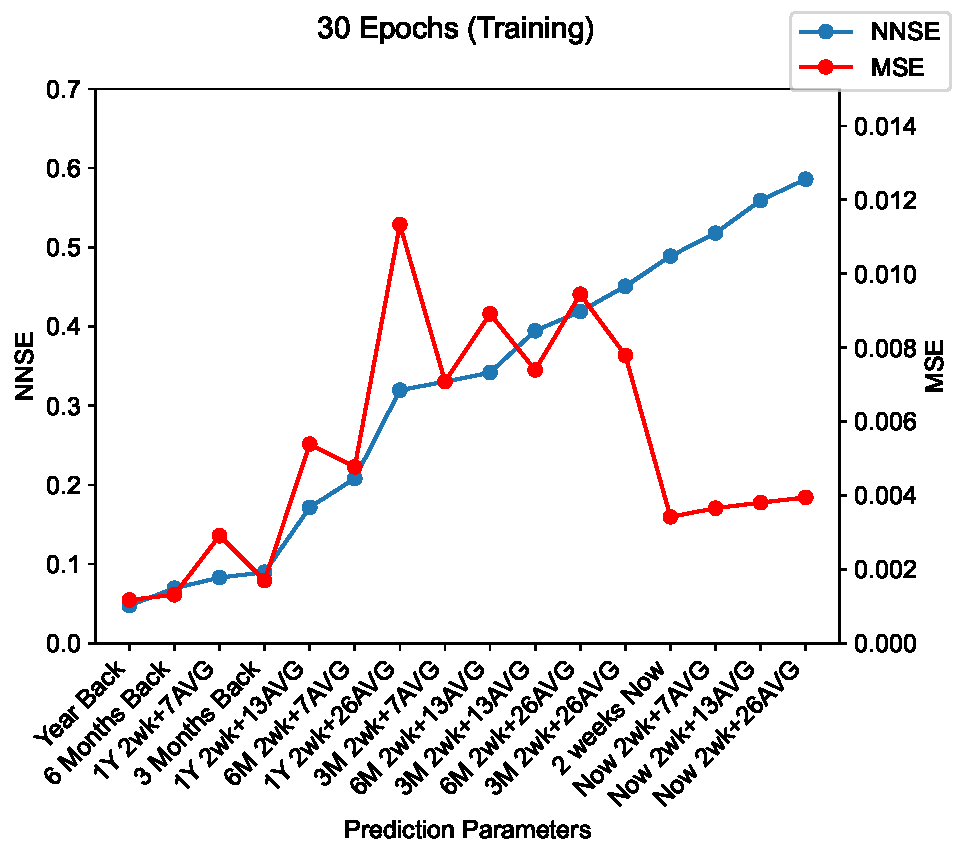
\includegraphics[width=1.0\linewidth]{images/30_training-MSE-and-NNSE.pdf}
        {\bf (C)} MSE and NNSE - 30 epochs training.
     \end{minipage}
     \ \
     \begin{minipage}[b]{0.45\textwidth}
        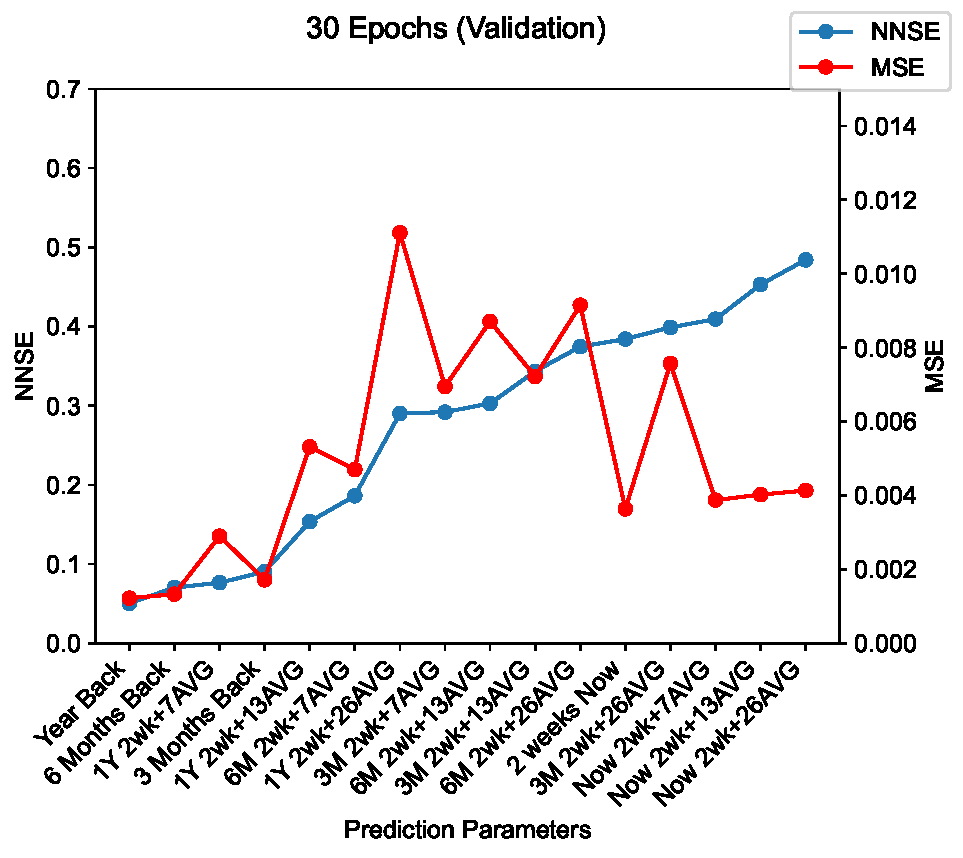
\includegraphics[width=1.0\linewidth]{images/30_validation-MSE-and-NNSE.pdf}
        {\bf (D)} MSE and NNSE - 30 epochs validation.
     \end{minipage}

     \begin{minipage}[b]{0.45\textwidth}
        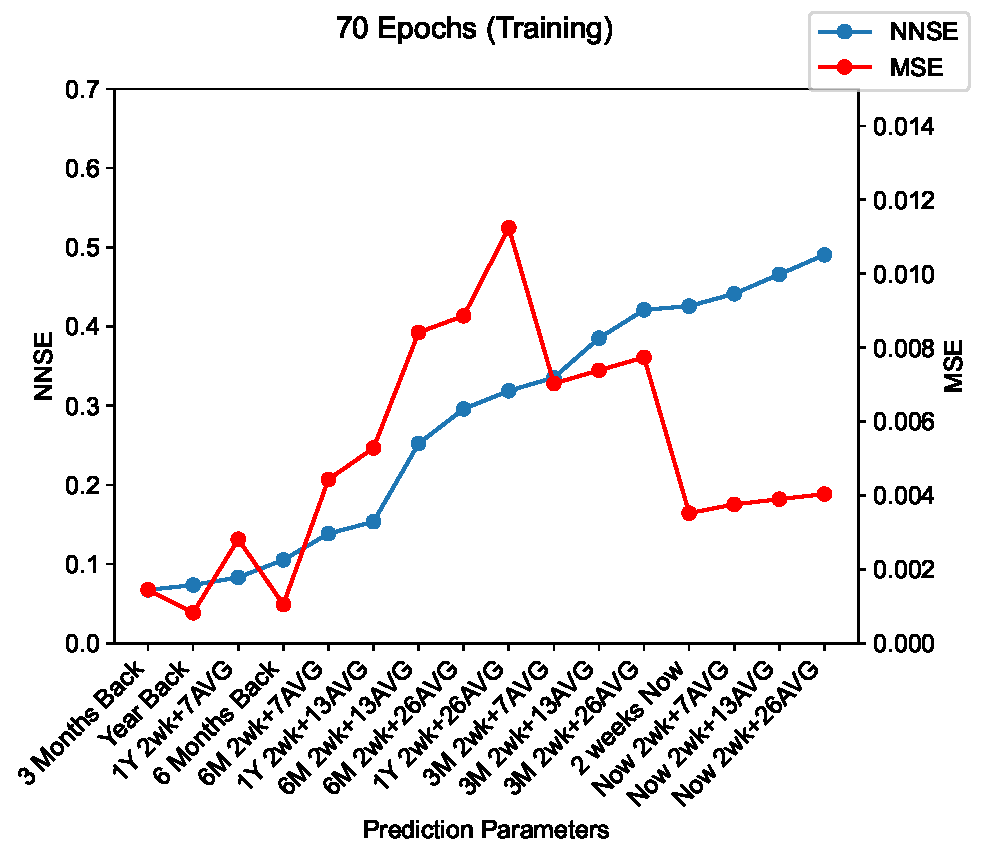
\includegraphics[width=1.0\linewidth]{images/70_training-MSE-and-NNSE.pdf}
        {\bf (E)} MSE and NNSE - 70 epochs training.
     \end{minipage}
     \ \
     \begin{minipage}[b]{0.45\textwidth}
        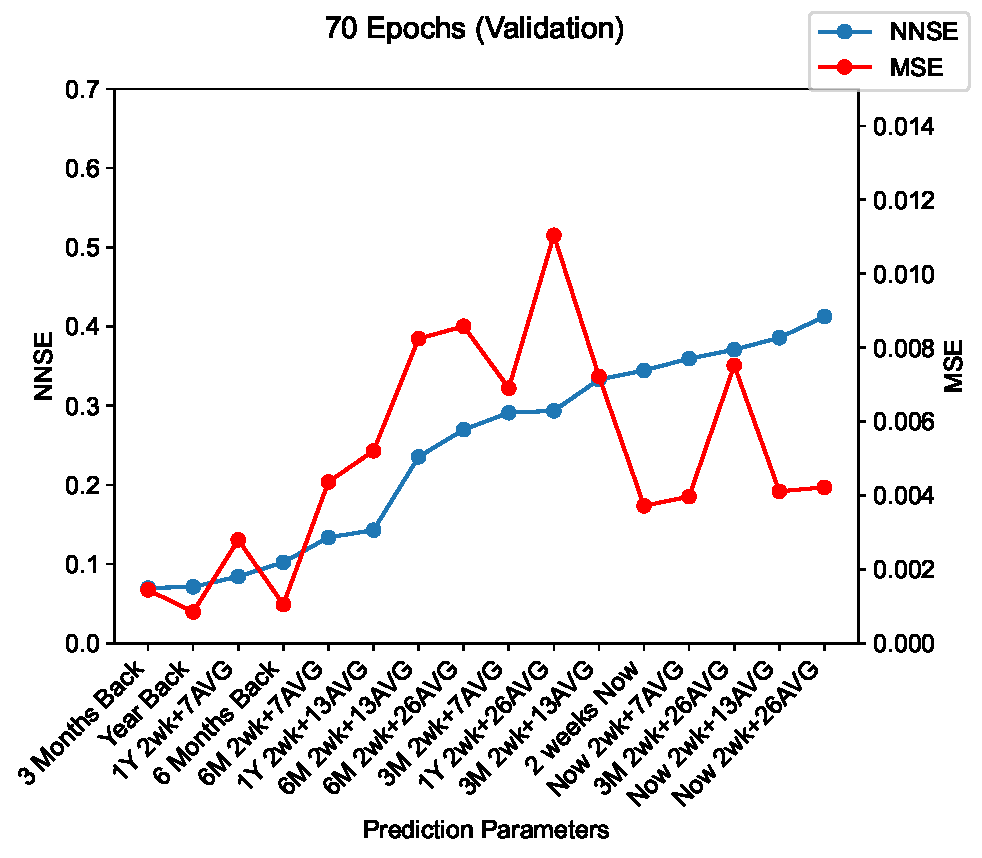
\includegraphics[width=1.0\linewidth]{images/70_validation-MSE-and-NNSE.pdf}
        {\bf (F)}  MSE and NNSE - 70 epochs validation.
     \end{minipage}
\end{center}

     \caption{NNSE and MSE values for training and validation for epochs 2 (A, B), 30 (C, D), 70 (E, F).}
     \label{fig:six graphs}
\end{figure}

%we have finalized the EQ code but want to make absolutely sure that we
%look at the correct values for the scientific comparison.
%
%This also requires a small sentence to each variable. Could we have a
%small meeting and I take then some notes on what these values are
%tomorrow. I will then add the explanations to the MLCommons EQ benchmark
%policy document.
%
%I just want to make sure I understand over which domain we average and
%sum up.
%
%Also if we were to just do one value (just in case they ask, I think we
%would use the summed up total right. However I think it is better to
%keep all of them.)
%
%Also I forgot what the +26 refers to
%
%I think something like this is almost correct, but we need to +26
%explanation and get verification from you.
%
%The Magnification based on a years worth of back data, while looking two
%weeks ahead + 26 what?

\begin{table}[p]

  \caption{Training and validation with time-based hyperparameters
    sorted by NNSE accuracy. The table includes the best two
    values highlighted in the training and validation results to
    showcase the accuracy of the validation. In the validation,
    we see that the best value for training is in rank four for the
    validation. The number of Epochs for this experiment is 2.
    26 is half of 52 and so 26 2-week intervals is a year.}
  \label{tab:training-2}

  \renewcommand{\arraystretch}{1.2}
  \begin{center}
    {\footnotesize
\begin{tabular}{|r|rl||rl|}
  \hline
{\bf Rank} & \multicolumn{2}{c||}{\bfseries Training} & \multicolumn{2}{c|}{\bfseries Validation}  \\
     &   {\bf NNSE} & {\bf Hyperparameters} & {\bf NNSE} & {\bf Hyperparameters} \\
\hline
1 & \color{red} 0.191300 & \color{red} Year Back & \color{blue} 0.195200 & \color{blue} 6M 2wk+7AVG \\
2 & 0.192700 & \color{blue} 6M 2wk+7AVG & \color{teal} 0.201000 & \color{teal} 6 Months Back \\
3 & 0.197000 & 6M 2wk+13AVG & 0.201600 & 6M 2wk+13AVG \\
4 & \color{teal} 0.201600 & \color{teal} 6 Months Back & \color{red} 0.204500 & \color{red} Year Back \\
5 & 0.232600 & 1Y 2wk+13AVG & 0.219700 & 3 Months Back \\
6 & 0.233000 & 3 Months Back & 0.228900 & 3M 2wk+7AVG \\
7 & 0.235800 & 1Y 2wk+7AVG & 0.238200 & 1Y 2wk+13AVG \\
8 & 0.243000 & 3M 2wk+7AVG & 0.249500 & 1Y 2wk+7AVG \\
9 & 0.251600 & 1Y 2wk+26AVG & 0.264400 & 6M 2wk+26AVG \\
10 & 0.251700 & 6M 2wk+26AVG & 0.266200 & 3M 2wk+13AVG \\
11 & 0.278800 & 3M 2wk+13AVG & 0.270300 & 1Y 2wk+26AVG \\
12 & 0.302500 & 3M 2wk+26AVG & 0.295800 & 3M 2wk+26AVG \\
13 & 0.405600 & Now 2wk+7AVG & 0.379700 & Now 2wk+7AVG \\
14 & 0.429900 & Now 2wk+13AVG & 0.412700 & Now 2wk+13AVG \\
15 & 0.506800 & 2 weeks Now & 0.470100 & 2 weeks Now \\
16 & 0.521800 & Now 2wk+26AVG & 0.502300 & Now 2wk+26AVG \\
\hline
\end{tabular}
}
\end{center}

%\end{table}

%\begin{table}[htb]

  \caption{Training and validation with time-based hyperparameters
    sorted by NNSE accuracy. The table includes the best two
    values highlighted in the training and validation results to
    showcase the accuracy of the validation. In the validation,
    we see that the best value for training is in rank four for the
    validation. The number of Epochs for this experiment is 30.
  }
  \label{tab:training-30}

  \renewcommand{\arraystretch}{1.2}
  \begin{center}
        {\footnotesize
\begin{tabular}{|r|rl||rl|}
\hline
{\bf Rank} &
\multicolumn{2}{c||}{\bfseries Training} &
\multicolumn{2}{c|}{\bfseries Validation} \\
     {\bf NNSE} &
     {\bf Hyperparameters} &
     {\bf NNSE} &
     {\bf Hyperparameters} \\
\hline
 1 & \color{red} 0.047600 & \color{red} Year Back & \color{red} 0.050500 & \color{red} Year Back \\
 2 & \color{blue} 0.069500 & \color{blue} 6 Months Back & \color{blue} 0.070300 & \color{blue} 6 Months Back \\
 3 & 0.082900 & 1Y 2wk+7AVG & 0.076500 & 1Y 2wk+7AVG \\
 4 & 0.089700 & 3 Months Back & 0.090400 & 3 Months Back \\
 5 & 0.171600 & 1Y 2wk+13AVG & 0.153600 & 1Y 2wk+13AVG \\
 6 & 0.208100 & 6M 2wk+7AVG & 0.186200 & 6M 2wk+7AVG \\
 7 & 0.319600 & 1Y 2wk+26AVG & 0.290100 & 1Y 2wk+26AVG \\
 8 & 0.330300 & 3M 2wk+7AVG & 0.291900 & 3M 2wk+7AVG \\
 9 & 0.341800 & 6M 2wk+13AVG & 0.302800 & 6M 2wk+13AVG \\
10 & 0.394600 & 3M 2wk+13AVG & 0.343400 & 3M 2wk+13AVG \\
11 & 0.418900 & 6M 2wk+26AVG & 0.374500 & 6M 2wk+26AVG \\
12 & 0.450800 & 3M 2wk+26AVG & 0.384100 & 2 weeks Now \\
13 & 0.488800 & 2 weeks Now & 0.398900 & 3M 2wk+26AVG \\
14 & 0.517900 & Now 2wk+7AVG & 0.409300 & Now 2wk+7AVG \\
15 & 0.559200 & Now 2wk+13AVG & 0.453000 & Now 2wk+13AVG \\
16 & 0.586000 & Now 2wk+26AVG & 0.484100 & Now 2wk+26AVG \\
\hline
\end{tabular}
}

\end{center}
\end{table}


\begin{table}[htb]

  \caption{Training and validation with time-based hyperparameters
    sorted by NNSE accuracy. The table includes the best two
    values highlighted in the training and validation results to
    showcase the accuracy of the validation. In the validation,
    we see that the best value for training is in rank four for the
    validation. The number of Epochs for this experiment is 70.}
  \label{tab:training-70}

  \renewcommand{\arraystretch}{1.2}
  \begin{center}
        {\footnotesize
\begin{tabular}{|r|rl||rl|}
  \hline
{\bf Rank} & \multicolumn{2}{c||}{\bfseries Training} & \multicolumn{2}{c|}{\bfseries Validation} \\
     &   {\bf NNSE} & {\bf Hyperparameters} & {\bf NNSE} & {\bf Hyperparameters} \\
              \hline
 1 & \color{red} 0.067400 & \color{red} 3 Months Back & \color{red}0.069800 & \color{red} 3 Months Back \\
 2 & \color{blue} 0.073500 & \color{blue} Year Back & \color{blue} 0.071200 & \color{blue} Year Back \\
 3 & 0.083100 & 1Y 2wk+7AVG & 0.084300 & 1Y 2wk+7AVG \\
 4 & 0.105300 & 6 Months Back & 0.102200 & 6 Months Back \\
 5 & 0.138400 & 6M 2wk+7AVG & 0.133700 & 6M 2wk+7AVG \\
 6 & 0.153500 & 1Y 2wk+13AVG & 0.142800 & 1Y 2wk+13AVG \\
 7 & 0.252100 & 6M 2wk+13AVG & 0.235400 & 6M 2wk+13AVG \\
 8 & 0.295900 & 6M 2wk+26AVG & 0.269700 & 6M 2wk+26AVG \\
 9 & 0.318800 & 1Y 2wk+26AVG & 0.291100 & 3M 2wk+7AVG \\
10 & 0.335400 & 3M 2wk+7AVG & 0.293500 & 1Y 2wk+26AVG \\
11 & 0.385200 & 3M 2wk+13AVG & 0.333000 & 3M 2wk+13AVG \\
12 & 0.421000 & 3M 2wk+26AVG & 0.344500 & 2 weeks Now \\
13 & 0.425700 & 2 weeks Now & 0.359400 & Now 2wk+7AVG \\
14 & 0.441300 & Now 2wk+7AVG & 0.370700 & 3M 2wk+26AVG \\
15 & 0.465800 & Now 2wk+13AVG & 0.385800 & Now 2wk+13AVG \\
16 & 0.490400 & Now 2wk+26AVG & 0.412500 & Now 2wk+26AVG \\
\hline
\end{tabular}
\end{center}
}

\end{table}


\subsection{Energy}
\label{sec:perf-energy}

\begin{figure}[htb]

  \begin{center}
     \begin{minipage}[t]{0.30\textwidth}
        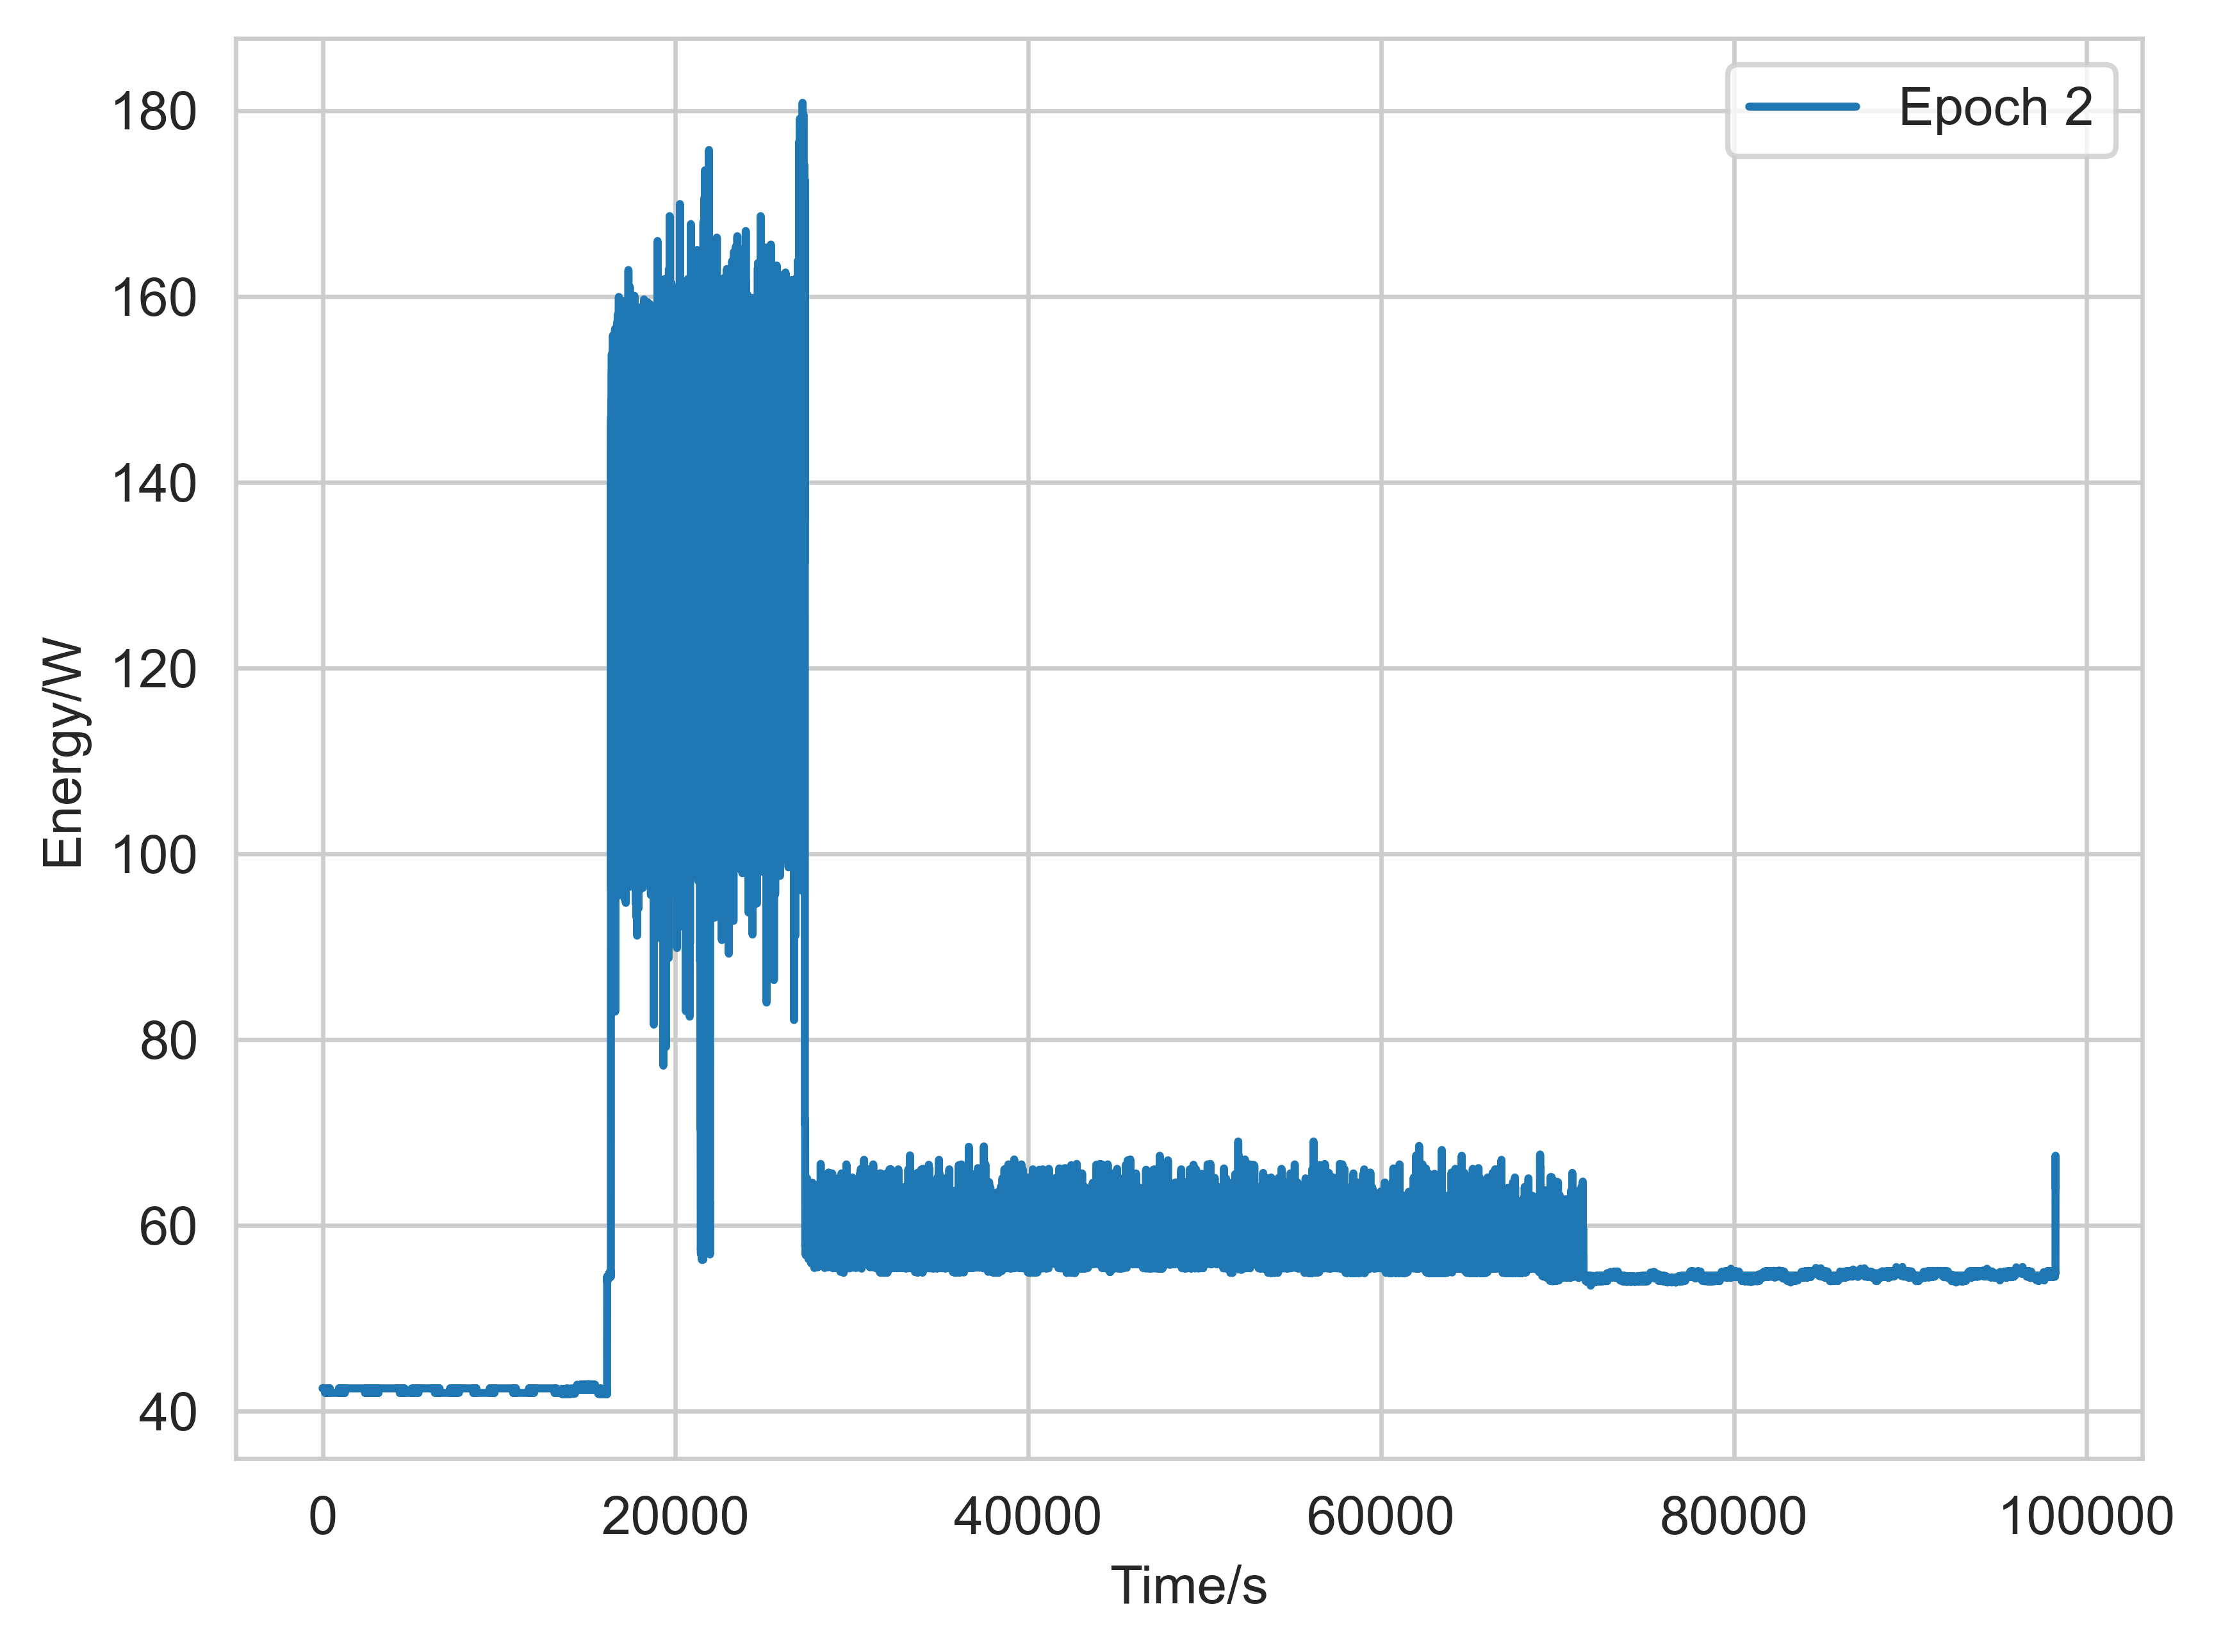
\includegraphics[width=1.0\linewidth]{images/card-name-v100-gpu-count-1-cpu-num-6-mem-32gb-repeat-1-tfttransformerepochs-2.png}
        {\bf (A)} Energy consumption for 2 epochs training and validation.
     \end{minipage}
     \ \
     \begin{minipage}[t]{0.30\textwidth}
        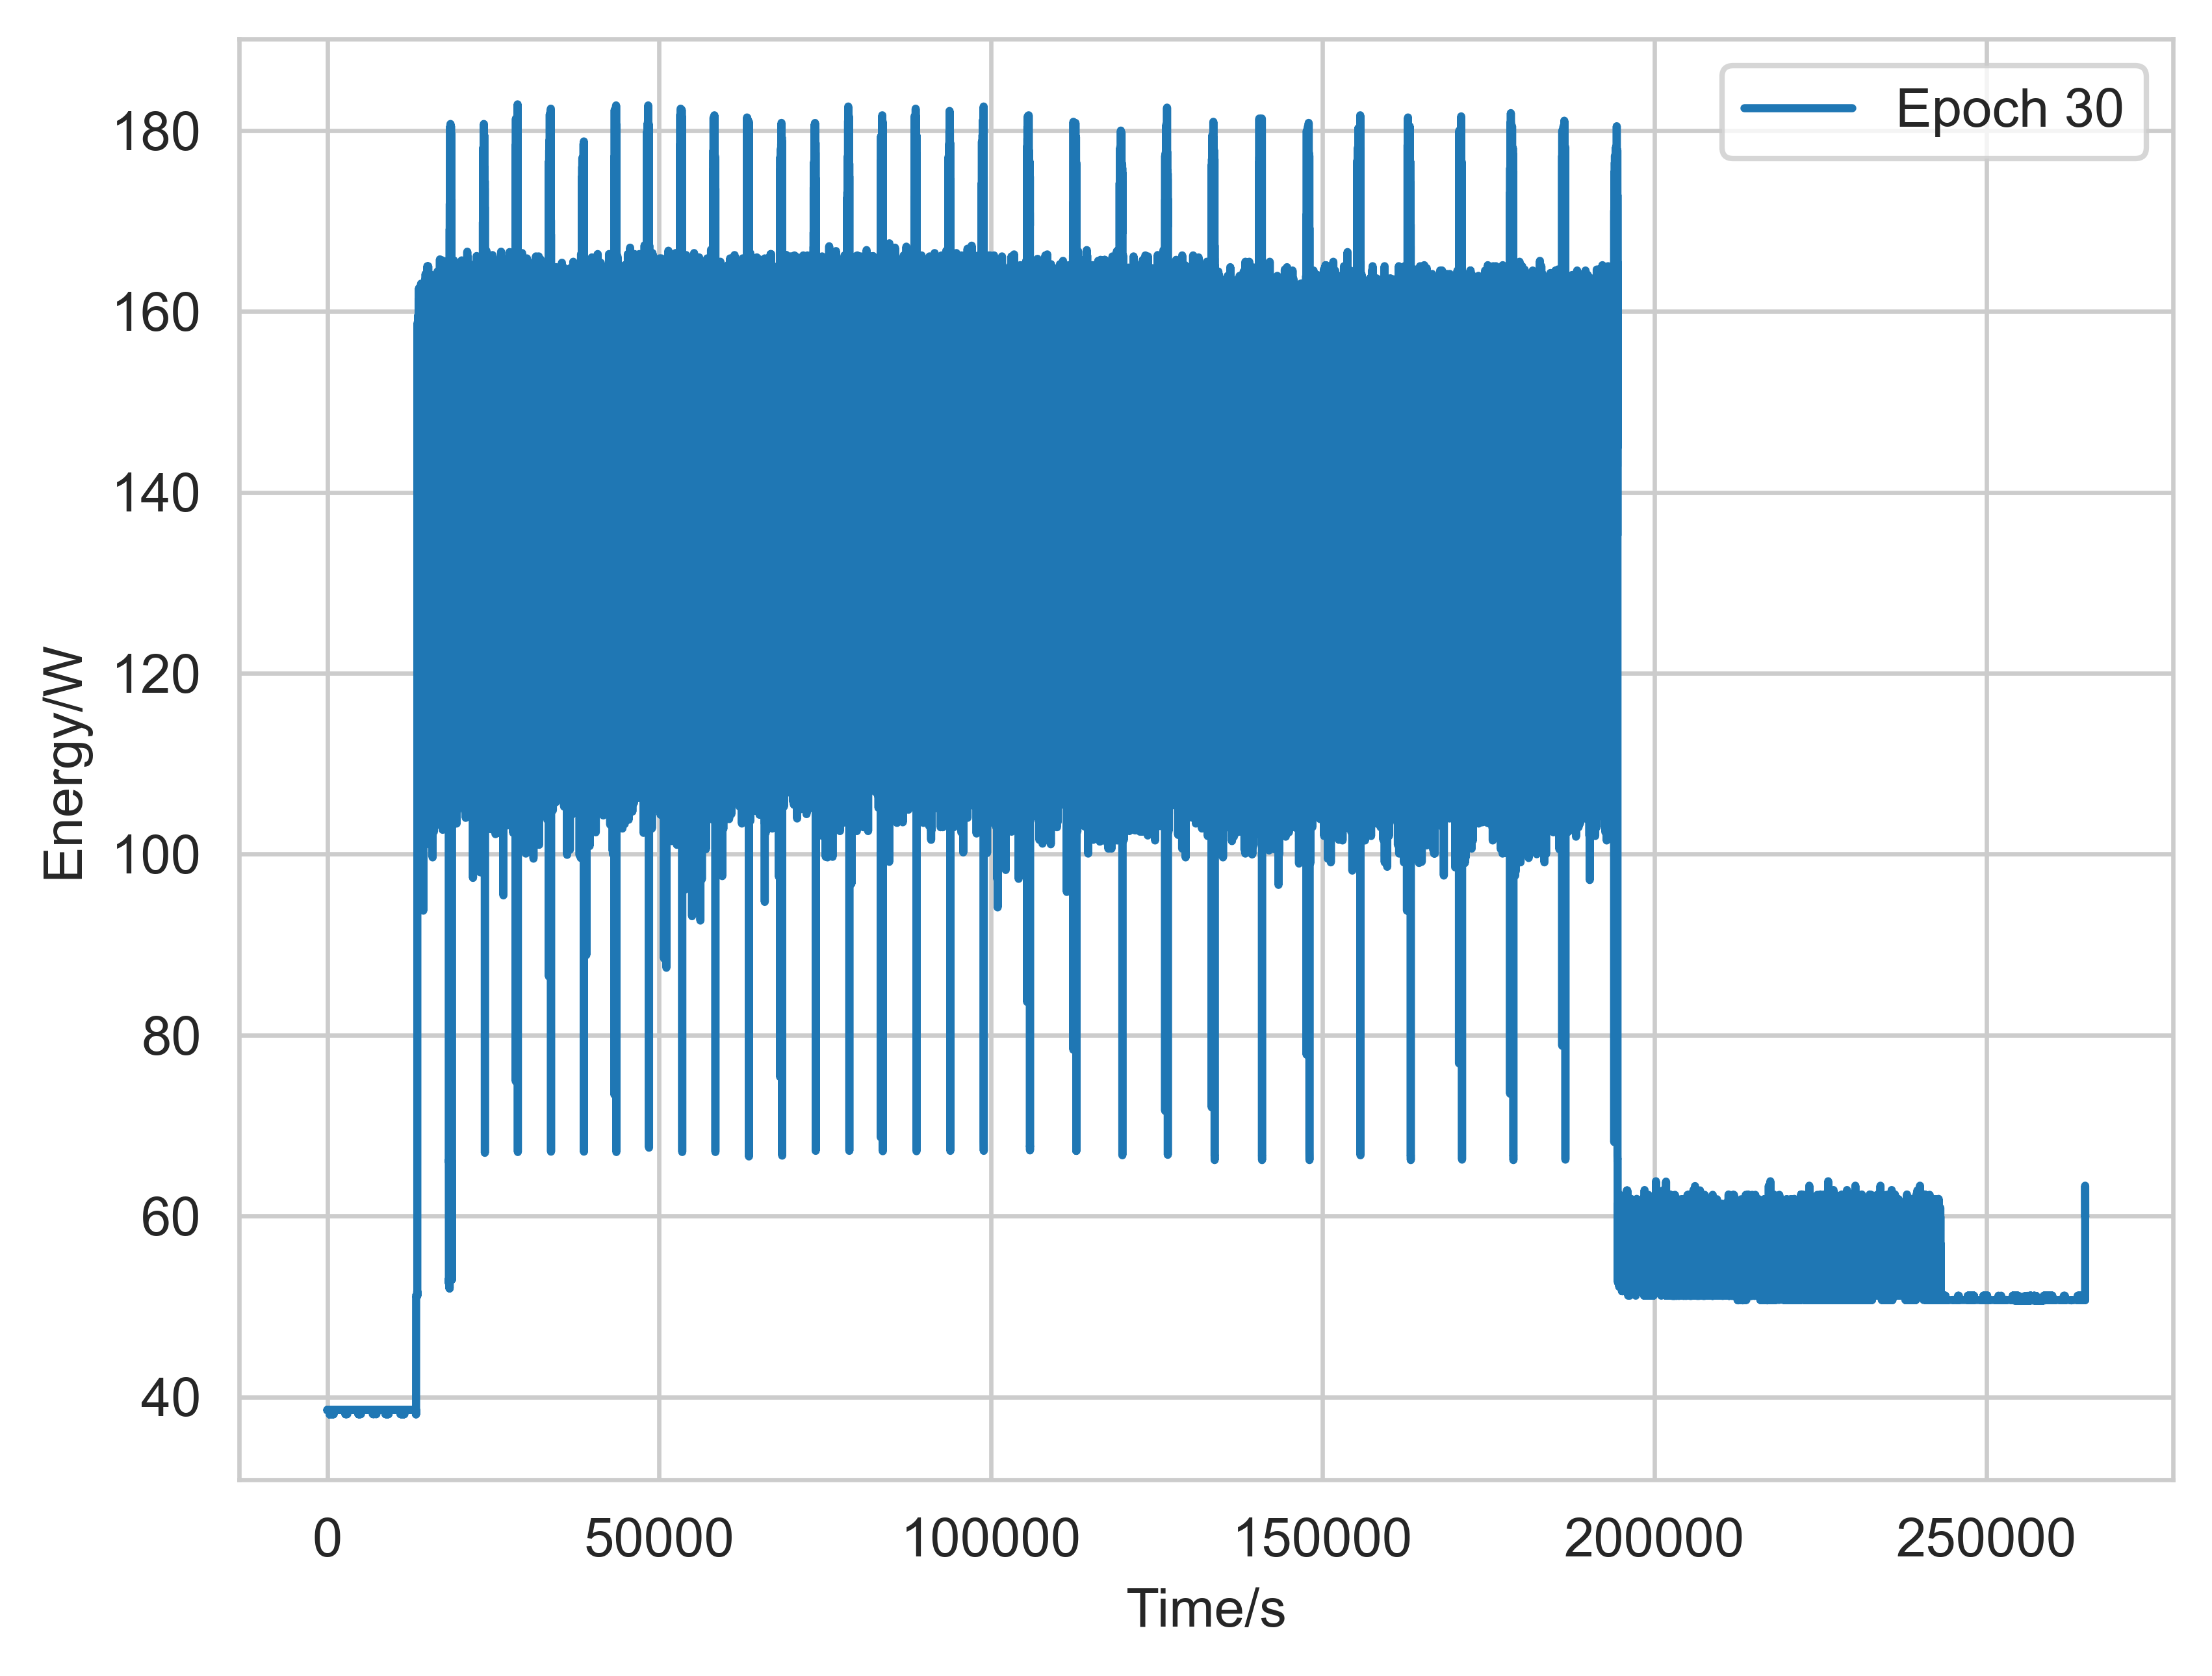
\includegraphics[width=1.0\linewidth]{images/card-name-v100-gpu-count-1-cpu-num-6-mem-32gb-repeat-1-tfttransformerepochs-30.png}
        {\bf (B)} Energy consumption for 30 epochs training and validation.
     \end{minipage}
     \ \
     \begin{minipage}[t]{0.30\textwidth}
        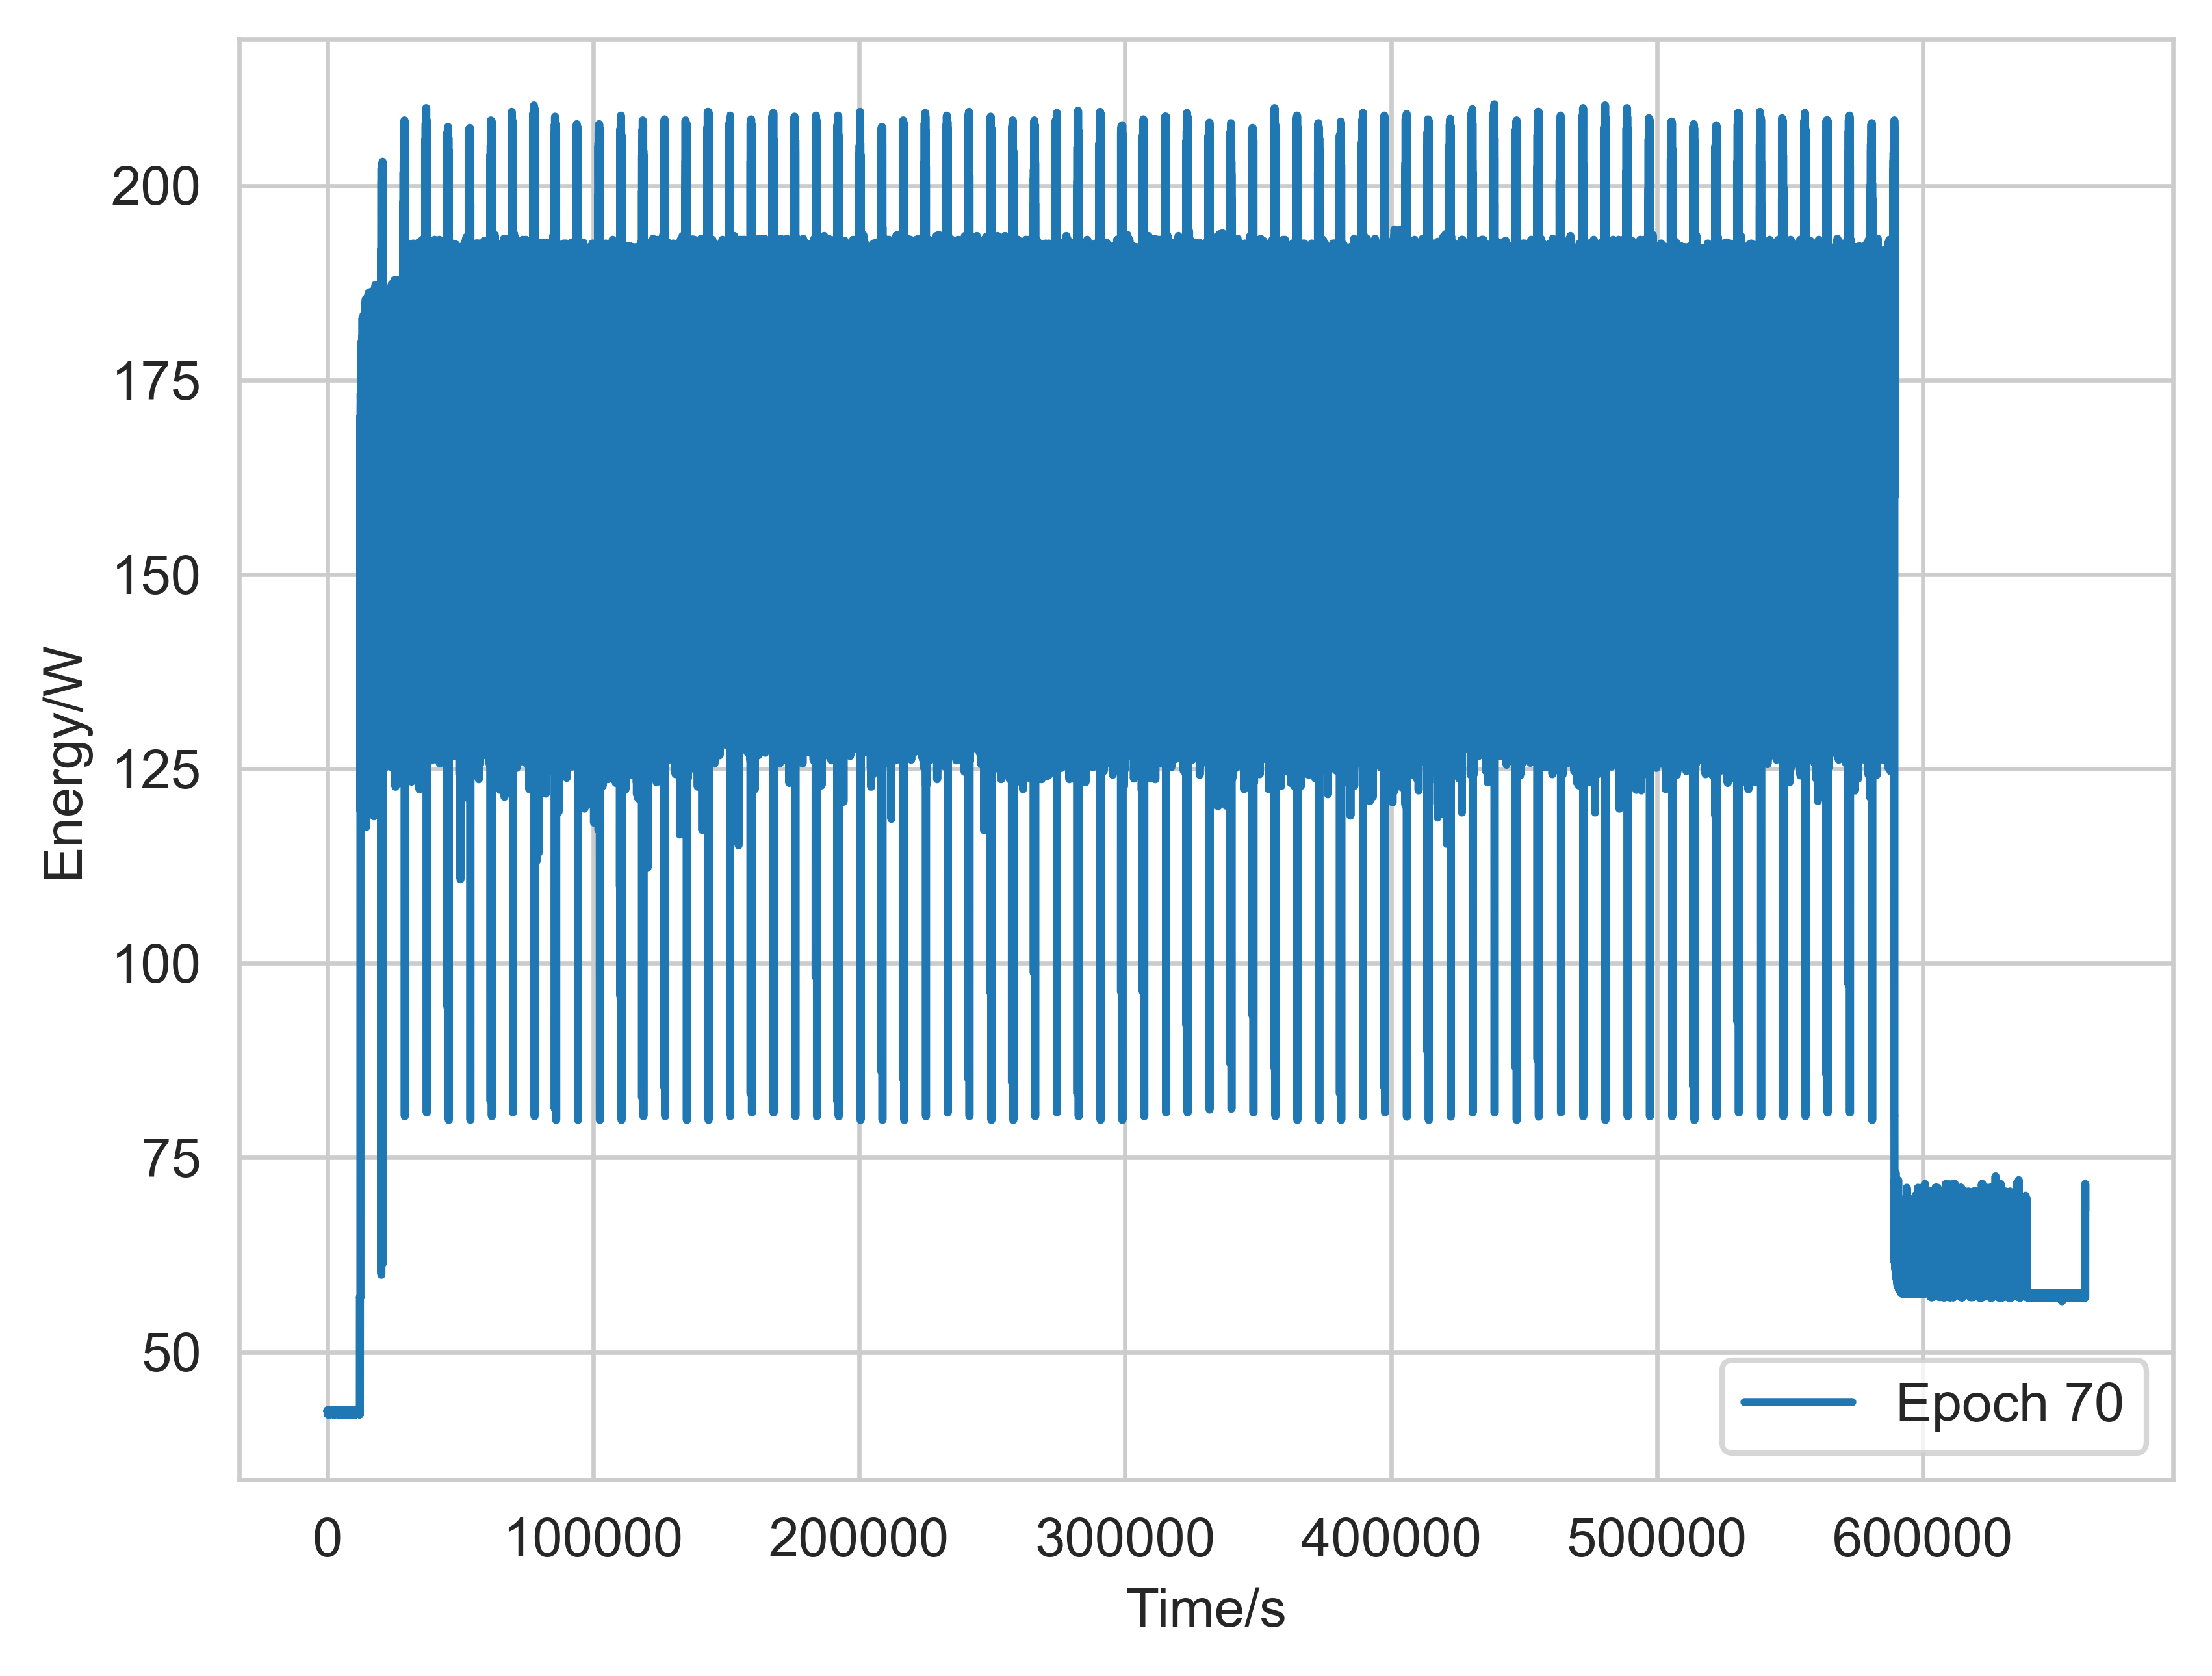
\includegraphics[width=1.0\linewidth]{images/card-name-v100-gpu-count-1-cpu-num-6-mem-32gb-repeat-1-tfttransformerepochs-70.png}
        {\bf (C)} Energy consumption for 70 epochs training and validation.
     \end{minipage}
  \end{center}

  \caption {Energy monitoring for 2, 30, and 70 epochs for training and validation.}
  \label{fig:energy}

\end{figure}

\begin{figure}[p]

  \begin{center}
     \begin{minipage}[t]{0.65\textwidth}
        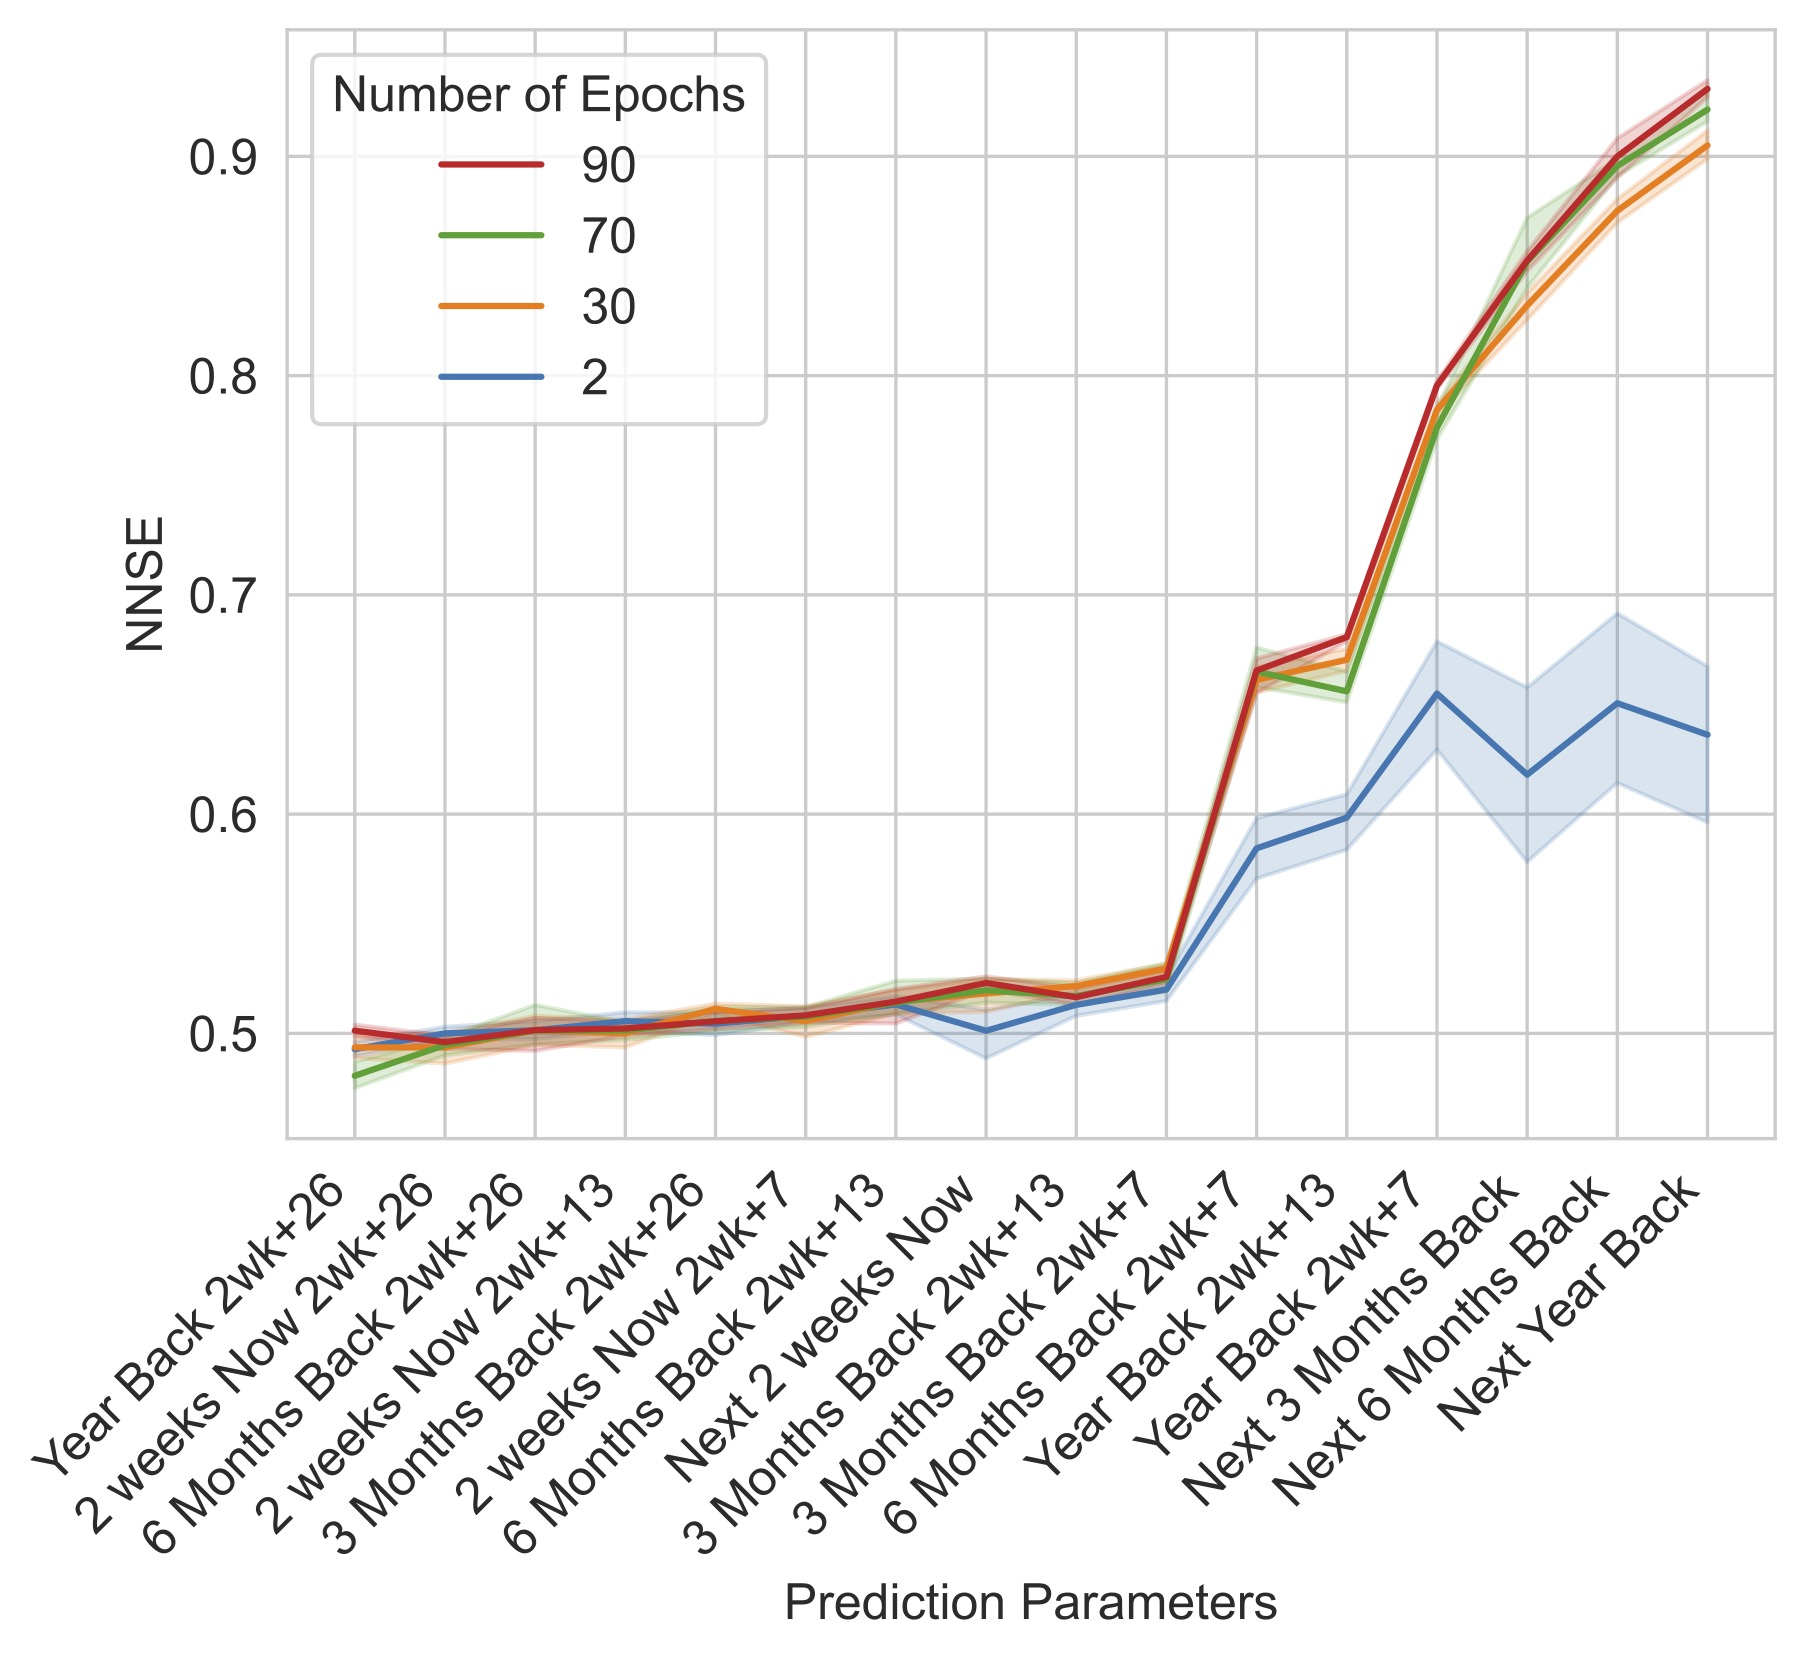
\includegraphics[width=1.0\linewidth]{images/NNSE-all-epochs-training}
        {\bf (A)} NNSE for training.
     \end{minipage}
  \end{center}
  \ \
  \begin{center}
     \begin{minipage}[t]{0.65\textwidth}
        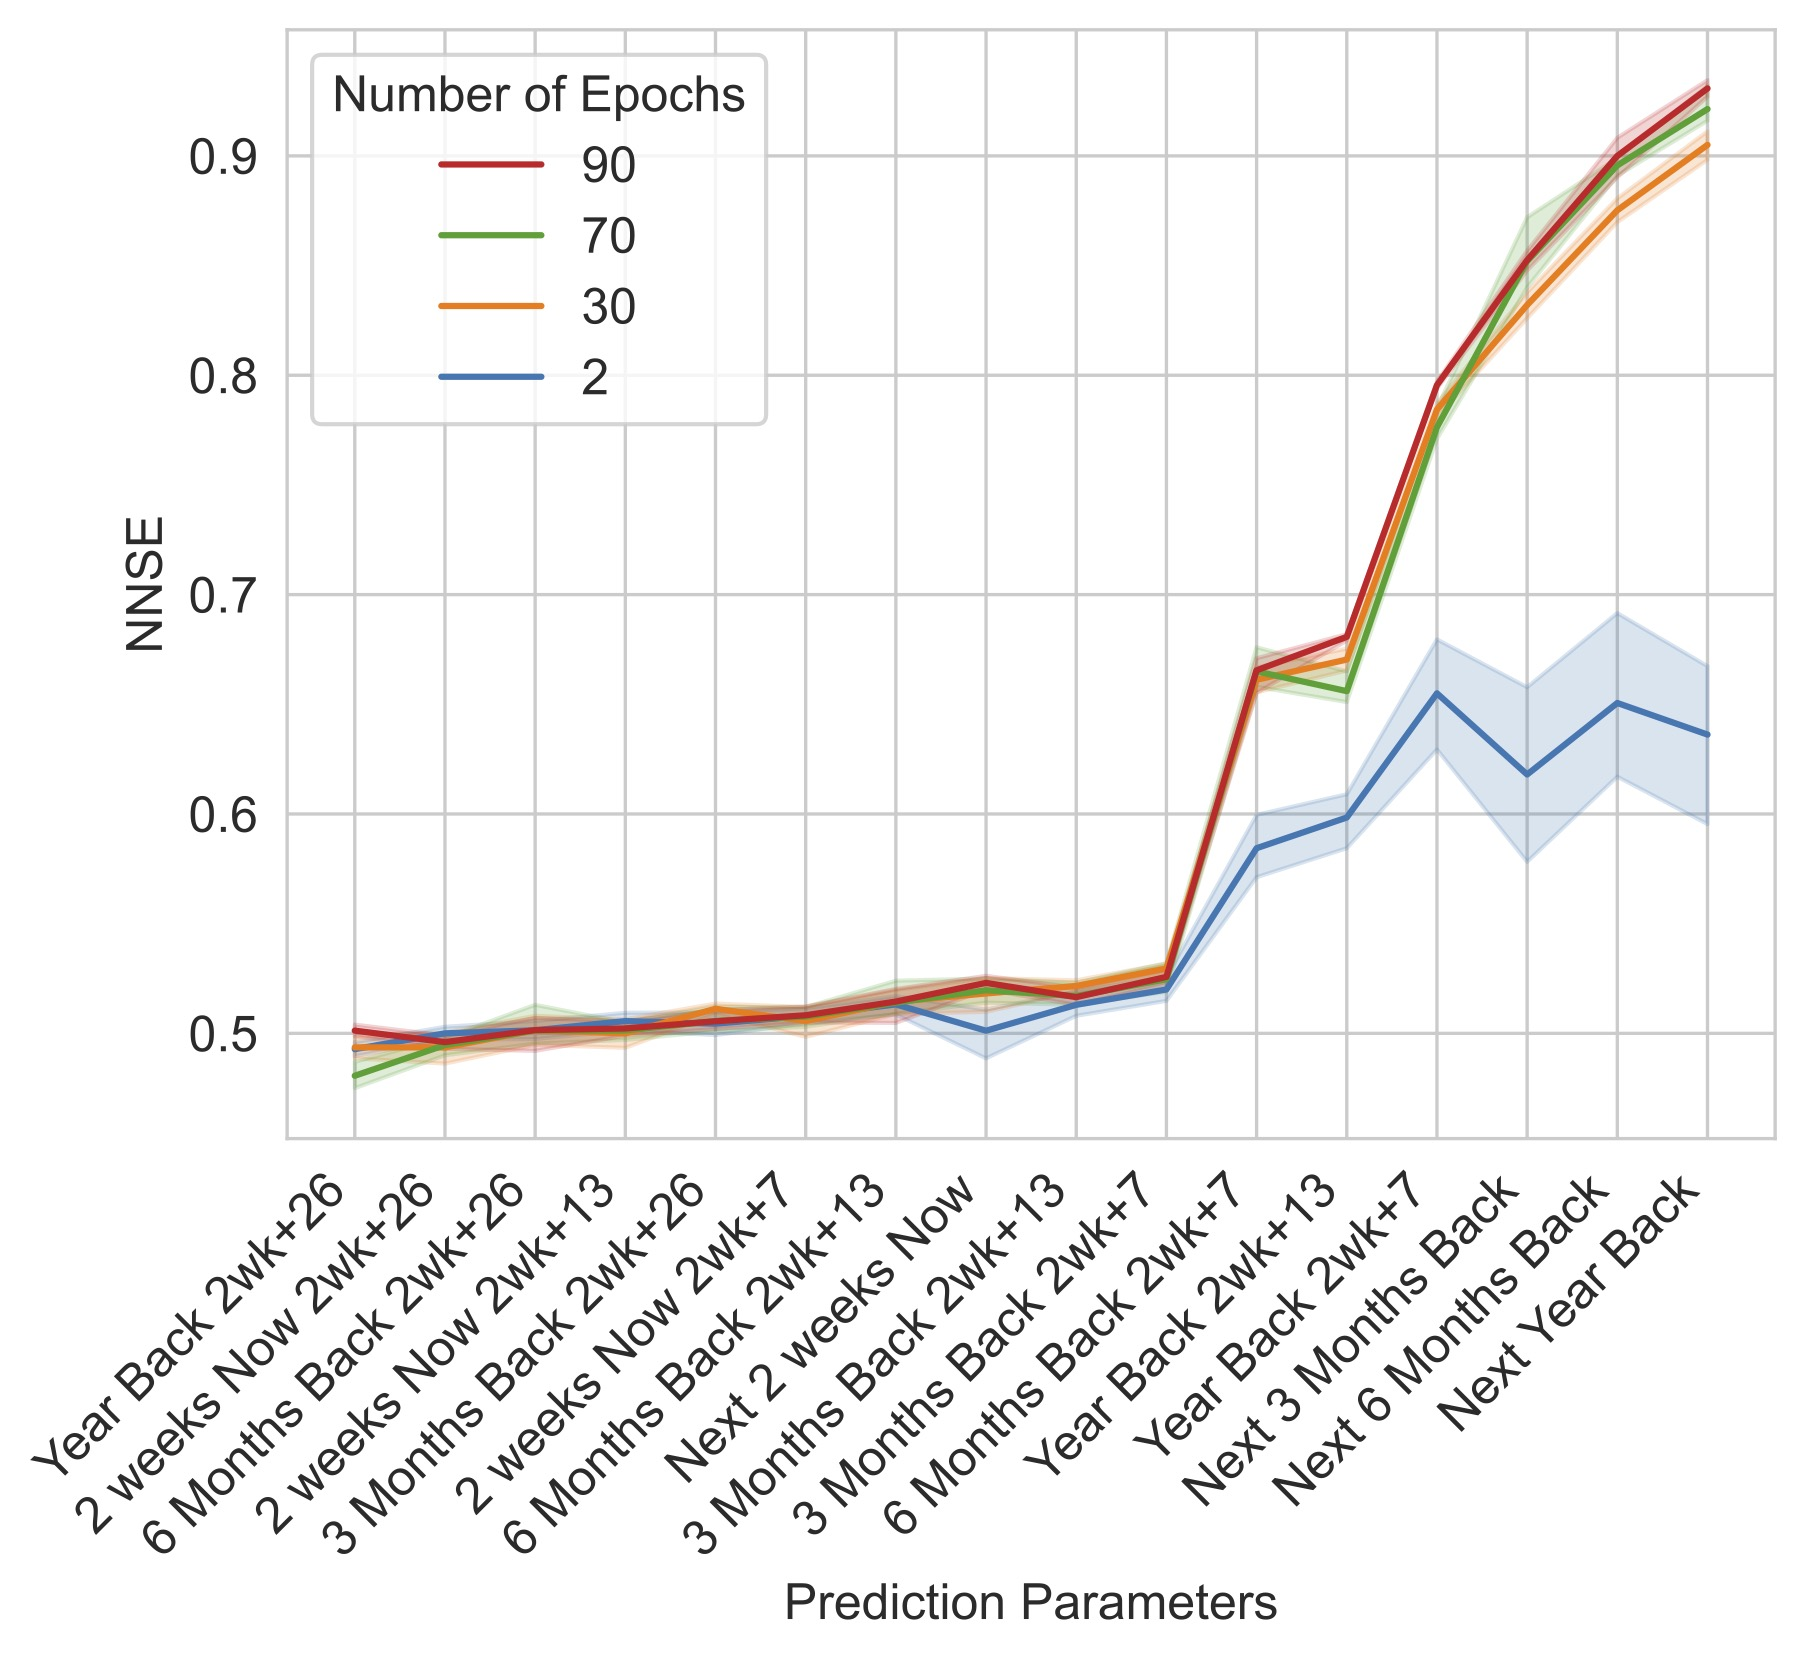
\includegraphics[width=1.0\linewidth]{images/NNSE-all-epochs-validation}
        {\bf (B)} NNSE for validation.
     \end{minipage}
  \end{center}

  \caption {NNSE comparison}
  \label{fig:NNSE-comparison}

\end{figure}

